% Created by tikzDevice version 0.10.1 on 2017-11-26 21:02:34
% !TEX encoding = UTF-8 Unicode
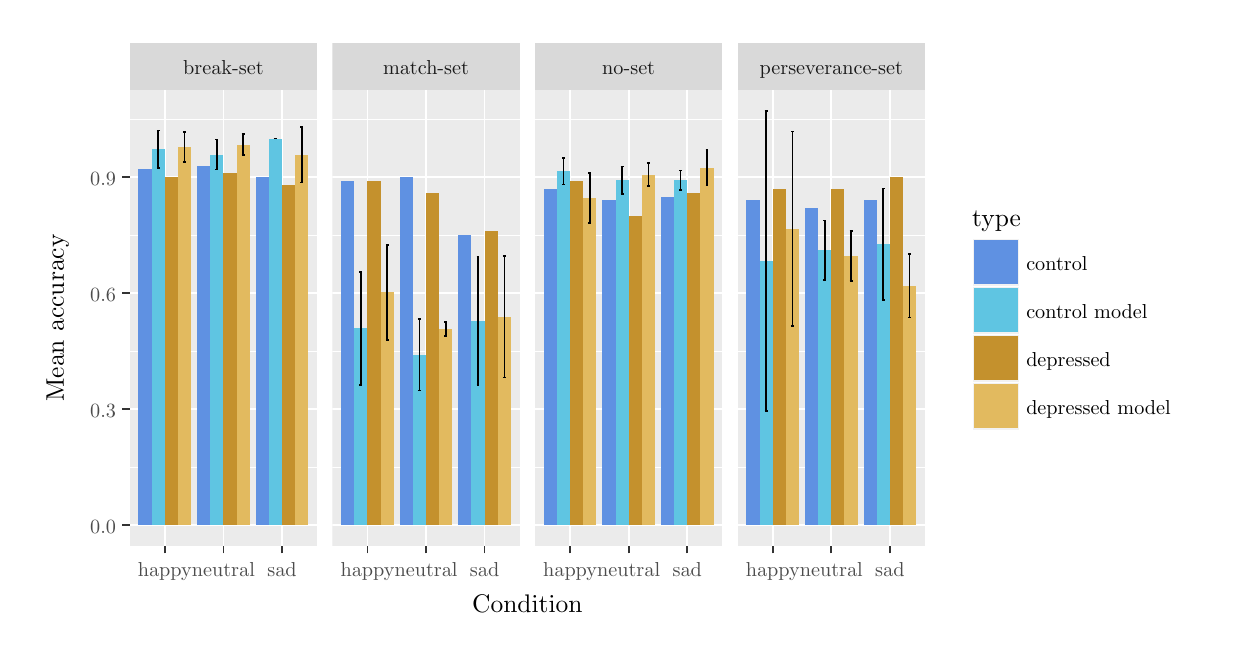
\begin{tikzpicture}[x=1pt,y=1pt]
\definecolor{fillColor}{RGB}{255,255,255}
\path[use as bounding box,fill=fillColor,fill opacity=0.00] (0,0) rectangle (433.62,216.81);
\begin{scope}
\path[clip] (  0.00,  0.00) rectangle (433.62,216.81);
\definecolor{drawColor}{RGB}{255,255,255}
\definecolor{fillColor}{RGB}{255,255,255}

\path[draw=drawColor,line width= 0.6pt,line join=round,line cap=round,fill=fillColor] (  0.00,  0.00) rectangle (433.62,216.81);
\end{scope}
\begin{scope}
\path[clip] ( 36.87, 29.59) rectangle (104.59,194.25);
\definecolor{fillColor}{gray}{0.92}

\path[fill=fillColor] ( 36.87, 29.59) rectangle (104.59,194.25);
\definecolor{drawColor}{RGB}{255,255,255}

\path[draw=drawColor,line width= 0.3pt,line join=round] ( 36.87, 58.02) --
	(104.59, 58.02);

\path[draw=drawColor,line width= 0.3pt,line join=round] ( 36.87, 99.93) --
	(104.59, 99.93);

\path[draw=drawColor,line width= 0.3pt,line join=round] ( 36.87,141.83) --
	(104.59,141.83);

\path[draw=drawColor,line width= 0.3pt,line join=round] ( 36.87,183.73) --
	(104.59,183.73);

\path[draw=drawColor,line width= 0.6pt,line join=round] ( 36.87, 37.07) --
	(104.59, 37.07);

\path[draw=drawColor,line width= 0.6pt,line join=round] ( 36.87, 78.97) --
	(104.59, 78.97);

\path[draw=drawColor,line width= 0.6pt,line join=round] ( 36.87,120.88) --
	(104.59,120.88);

\path[draw=drawColor,line width= 0.6pt,line join=round] ( 36.87,162.78) --
	(104.59,162.78);

\path[draw=drawColor,line width= 0.6pt,line join=round] ( 49.56, 29.59) --
	( 49.56,194.25);

\path[draw=drawColor,line width= 0.6pt,line join=round] ( 70.73, 29.59) --
	( 70.73,194.25);

\path[draw=drawColor,line width= 0.6pt,line join=round] ( 91.89, 29.59) --
	( 91.89,194.25);
\definecolor{fillColor}{RGB}{226,186,95}

\path[fill=fillColor] ( 54.33, 37.07) rectangle ( 59.09,173.65);
\definecolor{fillColor}{RGB}{196,145,45}

\path[fill=fillColor] ( 49.56, 37.07) rectangle ( 54.33,162.78);
\definecolor{fillColor}{RGB}{95,197,226}

\path[fill=fillColor] ( 44.80, 37.07) rectangle ( 49.56,172.87);
\definecolor{fillColor}{RGB}{95,145,226}

\path[fill=fillColor] ( 40.04, 37.07) rectangle ( 44.80,165.57);
\definecolor{fillColor}{RGB}{226,186,95}

\path[fill=fillColor] ( 75.49, 37.07) rectangle ( 80.25,174.53);
\definecolor{fillColor}{RGB}{196,145,45}

\path[fill=fillColor] ( 70.73, 37.07) rectangle ( 75.49,164.18);
\definecolor{fillColor}{RGB}{95,197,226}

\path[fill=fillColor] ( 65.97, 37.07) rectangle ( 70.73,170.95);
\definecolor{fillColor}{RGB}{95,145,226}

\path[fill=fillColor] ( 61.20, 37.07) rectangle ( 65.97,166.97);
\definecolor{fillColor}{RGB}{226,186,95}

\path[fill=fillColor] ( 96.65, 37.07) rectangle (101.41,170.93);
\definecolor{fillColor}{RGB}{196,145,45}

\path[fill=fillColor] ( 91.89, 37.07) rectangle ( 96.65,159.99);
\definecolor{fillColor}{RGB}{95,197,226}

\path[fill=fillColor] ( 87.13, 37.07) rectangle ( 91.89,176.75);
\definecolor{fillColor}{RGB}{95,145,226}

\path[fill=fillColor] ( 82.37, 37.07) rectangle ( 87.13,162.78);
\definecolor{drawColor}{RGB}{0,0,0}

\path[draw=drawColor,line width= 0.6pt,line join=round] ( 56.18,179.02) --
	( 57.24,179.02);

\path[draw=drawColor,line width= 0.6pt,line join=round] ( 56.71,179.02) --
	( 56.71,168.27);

\path[draw=drawColor,line width= 0.6pt,line join=round] ( 56.18,168.27) --
	( 57.24,168.27);

\path[draw=drawColor,line width= 0.6pt,line join=round] ( 46.65,179.59) --
	( 47.71,179.59);

\path[draw=drawColor,line width= 0.6pt,line join=round] ( 47.18,179.59) --
	( 47.18,166.15);

\path[draw=drawColor,line width= 0.6pt,line join=round] ( 46.65,166.15) --
	( 47.71,166.15);

\path[draw=drawColor,line width= 0.6pt,line join=round] ( 77.34,178.37) --
	( 78.40,178.37);

\path[draw=drawColor,line width= 0.6pt,line join=round] ( 77.87,178.37) --
	( 77.87,170.69);

\path[draw=drawColor,line width= 0.6pt,line join=round] ( 77.34,170.69) --
	( 78.40,170.69);

\path[draw=drawColor,line width= 0.6pt,line join=round] ( 67.82,176.37) --
	( 68.88,176.37);

\path[draw=drawColor,line width= 0.6pt,line join=round] ( 68.35,176.37) --
	( 68.35,165.53);

\path[draw=drawColor,line width= 0.6pt,line join=round] ( 67.82,165.53) --
	( 68.88,165.53);

\path[draw=drawColor,line width= 0.6pt,line join=round] ( 98.50,181.01) --
	( 99.56,181.01);

\path[draw=drawColor,line width= 0.6pt,line join=round] ( 99.03,181.01) --
	( 99.03,160.85);

\path[draw=drawColor,line width= 0.6pt,line join=round] ( 98.50,160.85) --
	( 99.56,160.85);

\path[draw=drawColor,line width= 0.6pt,line join=round] ( 88.98,176.75) --
	( 90.04,176.75);

\path[draw=drawColor,line width= 0.6pt,line join=round] ( 89.51,176.75) --
	( 89.51,176.75);

\path[draw=drawColor,line width= 0.6pt,line join=round] ( 88.98,176.75) --
	( 90.04,176.75);
\end{scope}
\begin{scope}
\path[clip] (110.09, 29.59) rectangle (177.81,194.25);
\definecolor{fillColor}{gray}{0.92}

\path[fill=fillColor] (110.09, 29.59) rectangle (177.81,194.25);
\definecolor{drawColor}{RGB}{255,255,255}

\path[draw=drawColor,line width= 0.3pt,line join=round] (110.09, 58.02) --
	(177.81, 58.02);

\path[draw=drawColor,line width= 0.3pt,line join=round] (110.09, 99.93) --
	(177.81, 99.93);

\path[draw=drawColor,line width= 0.3pt,line join=round] (110.09,141.83) --
	(177.81,141.83);

\path[draw=drawColor,line width= 0.3pt,line join=round] (110.09,183.73) --
	(177.81,183.73);

\path[draw=drawColor,line width= 0.6pt,line join=round] (110.09, 37.07) --
	(177.81, 37.07);

\path[draw=drawColor,line width= 0.6pt,line join=round] (110.09, 78.97) --
	(177.81, 78.97);

\path[draw=drawColor,line width= 0.6pt,line join=round] (110.09,120.88) --
	(177.81,120.88);

\path[draw=drawColor,line width= 0.6pt,line join=round] (110.09,162.78) --
	(177.81,162.78);

\path[draw=drawColor,line width= 0.6pt,line join=round] (122.79, 29.59) --
	(122.79,194.25);

\path[draw=drawColor,line width= 0.6pt,line join=round] (143.95, 29.59) --
	(143.95,194.25);

\path[draw=drawColor,line width= 0.6pt,line join=round] (165.11, 29.59) --
	(165.11,194.25);
\definecolor{fillColor}{RGB}{226,186,95}

\path[fill=fillColor] (127.55, 37.07) rectangle (132.31,121.12);
\definecolor{fillColor}{RGB}{196,145,45}

\path[fill=fillColor] (122.79, 37.07) rectangle (127.55,161.38);
\definecolor{fillColor}{RGB}{95,197,226}

\path[fill=fillColor] (118.02, 37.07) rectangle (122.79,108.15);
\definecolor{fillColor}{RGB}{95,145,226}

\path[fill=fillColor] (113.26, 37.07) rectangle (118.02,161.38);
\definecolor{fillColor}{RGB}{226,186,95}

\path[fill=fillColor] (148.71, 37.07) rectangle (153.47,107.93);
\definecolor{fillColor}{RGB}{196,145,45}

\path[fill=fillColor] (143.95, 37.07) rectangle (148.71,157.19);
\definecolor{fillColor}{RGB}{95,197,226}

\path[fill=fillColor] (139.19, 37.07) rectangle (143.95, 98.62);
\definecolor{fillColor}{RGB}{95,145,226}

\path[fill=fillColor] (134.43, 37.07) rectangle (139.19,162.78);
\definecolor{fillColor}{RGB}{226,186,95}

\path[fill=fillColor] (169.87, 37.07) rectangle (174.64,112.33);
\definecolor{fillColor}{RGB}{196,145,45}

\path[fill=fillColor] (165.11, 37.07) rectangle (169.87,143.23);
\definecolor{fillColor}{RGB}{95,197,226}

\path[fill=fillColor] (160.35, 37.07) rectangle (165.11,110.97);
\definecolor{fillColor}{RGB}{95,145,226}

\path[fill=fillColor] (155.59, 37.07) rectangle (160.35,141.83);
\definecolor{drawColor}{RGB}{0,0,0}

\path[draw=drawColor,line width= 0.6pt,line join=round] (129.40,138.23) --
	(130.46,138.23);

\path[draw=drawColor,line width= 0.6pt,line join=round] (129.93,138.23) --
	(129.93,104.02);

\path[draw=drawColor,line width= 0.6pt,line join=round] (129.40,104.02) --
	(130.46,104.02);

\path[draw=drawColor,line width= 0.6pt,line join=round] (119.88,128.62) --
	(120.93,128.62);

\path[draw=drawColor,line width= 0.6pt,line join=round] (120.40,128.62) --
	(120.40, 87.69);

\path[draw=drawColor,line width= 0.6pt,line join=round] (119.88, 87.69) --
	(120.93, 87.69);

\path[draw=drawColor,line width= 0.6pt,line join=round] (150.56,110.36) --
	(151.62,110.36);

\path[draw=drawColor,line width= 0.6pt,line join=round] (151.09,110.36) --
	(151.09,105.49);

\path[draw=drawColor,line width= 0.6pt,line join=round] (150.56,105.49) --
	(151.62,105.49);

\path[draw=drawColor,line width= 0.6pt,line join=round] (141.04,111.55) --
	(142.10,111.55);

\path[draw=drawColor,line width= 0.6pt,line join=round] (141.57,111.55) --
	(141.57, 85.68);

\path[draw=drawColor,line width= 0.6pt,line join=round] (141.04, 85.68) --
	(142.10, 85.68);

\path[draw=drawColor,line width= 0.6pt,line join=round] (171.73,134.22) --
	(172.78,134.22);

\path[draw=drawColor,line width= 0.6pt,line join=round] (172.25,134.22) --
	(172.25, 90.45);

\path[draw=drawColor,line width= 0.6pt,line join=round] (171.73, 90.45) --
	(172.78, 90.45);

\path[draw=drawColor,line width= 0.6pt,line join=round] (162.20,134.15) --
	(163.26,134.15);

\path[draw=drawColor,line width= 0.6pt,line join=round] (162.73,134.15) --
	(162.73, 87.80);

\path[draw=drawColor,line width= 0.6pt,line join=round] (162.20, 87.80) --
	(163.26, 87.80);
\end{scope}
\begin{scope}
\path[clip] (183.31, 29.59) rectangle (251.03,194.25);
\definecolor{fillColor}{gray}{0.92}

\path[fill=fillColor] (183.31, 29.59) rectangle (251.03,194.25);
\definecolor{drawColor}{RGB}{255,255,255}

\path[draw=drawColor,line width= 0.3pt,line join=round] (183.31, 58.02) --
	(251.03, 58.02);

\path[draw=drawColor,line width= 0.3pt,line join=round] (183.31, 99.93) --
	(251.03, 99.93);

\path[draw=drawColor,line width= 0.3pt,line join=round] (183.31,141.83) --
	(251.03,141.83);

\path[draw=drawColor,line width= 0.3pt,line join=round] (183.31,183.73) --
	(251.03,183.73);

\path[draw=drawColor,line width= 0.6pt,line join=round] (183.31, 37.07) --
	(251.03, 37.07);

\path[draw=drawColor,line width= 0.6pt,line join=round] (183.31, 78.97) --
	(251.03, 78.97);

\path[draw=drawColor,line width= 0.6pt,line join=round] (183.31,120.88) --
	(251.03,120.88);

\path[draw=drawColor,line width= 0.6pt,line join=round] (183.31,162.78) --
	(251.03,162.78);

\path[draw=drawColor,line width= 0.6pt,line join=round] (196.01, 29.59) --
	(196.01,194.25);

\path[draw=drawColor,line width= 0.6pt,line join=round] (217.17, 29.59) --
	(217.17,194.25);

\path[draw=drawColor,line width= 0.6pt,line join=round] (238.33, 29.59) --
	(238.33,194.25);
\definecolor{fillColor}{RGB}{226,186,95}

\path[fill=fillColor] (200.77, 37.07) rectangle (205.53,155.26);
\definecolor{fillColor}{RGB}{196,145,45}

\path[fill=fillColor] (196.01, 37.07) rectangle (200.77,161.38);
\definecolor{fillColor}{RGB}{95,197,226}

\path[fill=fillColor] (191.25, 37.07) rectangle (196.01,164.93);
\definecolor{fillColor}{RGB}{95,145,226}

\path[fill=fillColor] (186.48, 37.07) rectangle (191.25,158.59);
\definecolor{fillColor}{RGB}{226,186,95}

\path[fill=fillColor] (221.93, 37.07) rectangle (226.69,163.74);
\definecolor{fillColor}{RGB}{196,145,45}

\path[fill=fillColor] (217.17, 37.07) rectangle (221.93,148.81);
\definecolor{fillColor}{RGB}{95,197,226}

\path[fill=fillColor] (212.41, 37.07) rectangle (217.17,161.69);
\definecolor{fillColor}{RGB}{95,145,226}

\path[fill=fillColor] (207.65, 37.07) rectangle (212.41,154.40);
\definecolor{fillColor}{RGB}{226,186,95}

\path[fill=fillColor] (243.10, 37.07) rectangle (247.86,166.18);
\definecolor{fillColor}{RGB}{196,145,45}

\path[fill=fillColor] (238.33, 37.07) rectangle (243.10,157.19);
\definecolor{fillColor}{RGB}{95,197,226}

\path[fill=fillColor] (233.57, 37.07) rectangle (238.33,161.72);
\definecolor{fillColor}{RGB}{95,145,226}

\path[fill=fillColor] (228.81, 37.07) rectangle (233.57,155.80);
\definecolor{drawColor}{RGB}{0,0,0}

\path[draw=drawColor,line width= 0.6pt,line join=round] (202.62,164.34) --
	(203.68,164.34);

\path[draw=drawColor,line width= 0.6pt,line join=round] (203.15,164.34) --
	(203.15,146.18);

\path[draw=drawColor,line width= 0.6pt,line join=round] (202.62,146.18) --
	(203.68,146.18);

\path[draw=drawColor,line width= 0.6pt,line join=round] (193.10,169.67) --
	(194.16,169.67);

\path[draw=drawColor,line width= 0.6pt,line join=round] (193.63,169.67) --
	(193.63,160.18);

\path[draw=drawColor,line width= 0.6pt,line join=round] (193.10,160.18) --
	(194.16,160.18);

\path[draw=drawColor,line width= 0.6pt,line join=round] (223.78,167.93) --
	(224.84,167.93);

\path[draw=drawColor,line width= 0.6pt,line join=round] (224.31,167.93) --
	(224.31,159.55);

\path[draw=drawColor,line width= 0.6pt,line join=round] (223.78,159.55) --
	(224.84,159.55);

\path[draw=drawColor,line width= 0.6pt,line join=round] (214.26,166.68) --
	(215.32,166.68);

\path[draw=drawColor,line width= 0.6pt,line join=round] (214.79,166.68) --
	(214.79,156.70);

\path[draw=drawColor,line width= 0.6pt,line join=round] (214.26,156.70) --
	(215.32,156.70);

\path[draw=drawColor,line width= 0.6pt,line join=round] (244.95,172.62) --
	(246.01,172.62);

\path[draw=drawColor,line width= 0.6pt,line join=round] (245.48,172.62) --
	(245.48,159.75);

\path[draw=drawColor,line width= 0.6pt,line join=round] (244.95,159.75) --
	(246.01,159.75);

\path[draw=drawColor,line width= 0.6pt,line join=round] (235.42,165.19) --
	(236.48,165.19);

\path[draw=drawColor,line width= 0.6pt,line join=round] (235.95,165.19) --
	(235.95,158.25);

\path[draw=drawColor,line width= 0.6pt,line join=round] (235.42,158.25) --
	(236.48,158.25);
\end{scope}
\begin{scope}
\path[clip] (256.53, 29.59) rectangle (324.25,194.25);
\definecolor{fillColor}{gray}{0.92}

\path[fill=fillColor] (256.53, 29.59) rectangle (324.25,194.25);
\definecolor{drawColor}{RGB}{255,255,255}

\path[draw=drawColor,line width= 0.3pt,line join=round] (256.53, 58.02) --
	(324.25, 58.02);

\path[draw=drawColor,line width= 0.3pt,line join=round] (256.53, 99.93) --
	(324.25, 99.93);

\path[draw=drawColor,line width= 0.3pt,line join=round] (256.53,141.83) --
	(324.25,141.83);

\path[draw=drawColor,line width= 0.3pt,line join=round] (256.53,183.73) --
	(324.25,183.73);

\path[draw=drawColor,line width= 0.6pt,line join=round] (256.53, 37.07) --
	(324.25, 37.07);

\path[draw=drawColor,line width= 0.6pt,line join=round] (256.53, 78.97) --
	(324.25, 78.97);

\path[draw=drawColor,line width= 0.6pt,line join=round] (256.53,120.88) --
	(324.25,120.88);

\path[draw=drawColor,line width= 0.6pt,line join=round] (256.53,162.78) --
	(324.25,162.78);

\path[draw=drawColor,line width= 0.6pt,line join=round] (269.23, 29.59) --
	(269.23,194.25);

\path[draw=drawColor,line width= 0.6pt,line join=round] (290.39, 29.59) --
	(290.39,194.25);

\path[draw=drawColor,line width= 0.6pt,line join=round] (311.56, 29.59) --
	(311.56,194.25);
\definecolor{fillColor}{RGB}{226,186,95}

\path[fill=fillColor] (273.99, 37.07) rectangle (278.75,144.16);
\definecolor{fillColor}{RGB}{196,145,45}

\path[fill=fillColor] (269.23, 37.07) rectangle (273.99,158.59);
\definecolor{fillColor}{RGB}{95,197,226}

\path[fill=fillColor] (264.47, 37.07) rectangle (269.23,132.52);
\definecolor{fillColor}{RGB}{95,145,226}

\path[fill=fillColor] (259.71, 37.07) rectangle (264.47,154.40);
\definecolor{fillColor}{RGB}{226,186,95}

\path[fill=fillColor] (295.15, 37.07) rectangle (299.92,134.35);
\definecolor{fillColor}{RGB}{196,145,45}

\path[fill=fillColor] (290.39, 37.07) rectangle (295.15,158.59);
\definecolor{fillColor}{RGB}{95,197,226}

\path[fill=fillColor] (285.63, 37.07) rectangle (290.39,136.40);
\definecolor{fillColor}{RGB}{95,145,226}

\path[fill=fillColor] (280.87, 37.07) rectangle (285.63,151.61);
\definecolor{fillColor}{RGB}{226,186,95}

\path[fill=fillColor] (316.32, 37.07) rectangle (321.08,123.54);
\definecolor{fillColor}{RGB}{196,145,45}

\path[fill=fillColor] (311.56, 37.07) rectangle (316.32,162.78);
\definecolor{fillColor}{RGB}{95,197,226}

\path[fill=fillColor] (306.79, 37.07) rectangle (311.56,138.50);
\definecolor{fillColor}{RGB}{95,145,226}

\path[fill=fillColor] (302.03, 37.07) rectangle (306.79,154.40);
\definecolor{drawColor}{RGB}{0,0,0}

\path[draw=drawColor,line width= 0.6pt,line join=round] (275.84,179.31) --
	(276.90,179.31);

\path[draw=drawColor,line width= 0.6pt,line join=round] (276.37,179.31) --
	(276.37,109.01);

\path[draw=drawColor,line width= 0.6pt,line join=round] (275.84,109.01) --
	(276.90,109.01);

\path[draw=drawColor,line width= 0.6pt,line join=round] (266.32,186.76) --
	(267.38,186.76);

\path[draw=drawColor,line width= 0.6pt,line join=round] (266.85,186.76) --
	(266.85, 78.27);

\path[draw=drawColor,line width= 0.6pt,line join=round] (266.32, 78.27) --
	(267.38, 78.27);

\path[draw=drawColor,line width= 0.6pt,line join=round] (297.01,143.34) --
	(298.06,143.34);

\path[draw=drawColor,line width= 0.6pt,line join=round] (297.53,143.34) --
	(297.53,125.35);

\path[draw=drawColor,line width= 0.6pt,line join=round] (297.01,125.35) --
	(298.06,125.35);

\path[draw=drawColor,line width= 0.6pt,line join=round] (287.48,147.15) --
	(288.54,147.15);

\path[draw=drawColor,line width= 0.6pt,line join=round] (288.01,147.15) --
	(288.01,125.65);

\path[draw=drawColor,line width= 0.6pt,line join=round] (287.48,125.65) --
	(288.54,125.65);

\path[draw=drawColor,line width= 0.6pt,line join=round] (318.17,135.06) --
	(319.23,135.06);

\path[draw=drawColor,line width= 0.6pt,line join=round] (318.70,135.06) --
	(318.70,112.02);

\path[draw=drawColor,line width= 0.6pt,line join=round] (318.17,112.02) --
	(319.23,112.02);

\path[draw=drawColor,line width= 0.6pt,line join=round] (308.65,158.66) --
	(309.70,158.66);

\path[draw=drawColor,line width= 0.6pt,line join=round] (309.17,158.66) --
	(309.17,118.34);

\path[draw=drawColor,line width= 0.6pt,line join=round] (308.65,118.34) --
	(309.70,118.34);
\end{scope}
\begin{scope}
\path[clip] ( 36.87,194.25) rectangle (104.59,211.31);
\definecolor{fillColor}{gray}{0.85}

\path[fill=fillColor] ( 36.87,194.25) rectangle (104.59,211.31);
\definecolor{drawColor}{gray}{0.10}

\node[text=drawColor,anchor=base,inner sep=0pt, outer sep=0pt, scale=  0.73] at ( 70.73,199.75) {break-set};
\end{scope}
\begin{scope}
\path[clip] (110.09,194.25) rectangle (177.81,211.31);
\definecolor{fillColor}{gray}{0.85}

\path[fill=fillColor] (110.09,194.25) rectangle (177.81,211.31);
\definecolor{drawColor}{gray}{0.10}

\node[text=drawColor,anchor=base,inner sep=0pt, outer sep=0pt, scale=  0.73] at (143.95,199.75) {match-set};
\end{scope}
\begin{scope}
\path[clip] (183.31,194.25) rectangle (251.03,211.31);
\definecolor{fillColor}{gray}{0.85}

\path[fill=fillColor] (183.31,194.25) rectangle (251.03,211.31);
\definecolor{drawColor}{gray}{0.10}

\node[text=drawColor,anchor=base,inner sep=0pt, outer sep=0pt, scale=  0.73] at (217.17,199.75) {no-set};
\end{scope}
\begin{scope}
\path[clip] (256.53,194.25) rectangle (324.25,211.31);
\definecolor{fillColor}{gray}{0.85}

\path[fill=fillColor] (256.53,194.25) rectangle (324.25,211.31);
\definecolor{drawColor}{gray}{0.10}

\node[text=drawColor,anchor=base,inner sep=0pt, outer sep=0pt, scale=  0.73] at (290.39,199.75) {perseverance-set};
\end{scope}
\begin{scope}
\path[clip] (  0.00,  0.00) rectangle (433.62,216.81);
\definecolor{drawColor}{gray}{0.20}

\path[draw=drawColor,line width= 0.6pt,line join=round] ( 49.56, 26.84) --
	( 49.56, 29.59);

\path[draw=drawColor,line width= 0.6pt,line join=round] ( 70.73, 26.84) --
	( 70.73, 29.59);

\path[draw=drawColor,line width= 0.6pt,line join=round] ( 91.89, 26.84) --
	( 91.89, 29.59);
\end{scope}
\begin{scope}
\path[clip] (  0.00,  0.00) rectangle (433.62,216.81);
\definecolor{drawColor}{gray}{0.30}

\node[text=drawColor,anchor=base,inner sep=0pt, outer sep=0pt, scale=  0.73] at ( 49.56, 18.58) {happy};

\node[text=drawColor,anchor=base,inner sep=0pt, outer sep=0pt, scale=  0.73] at ( 70.73, 18.58) {neutral};

\node[text=drawColor,anchor=base,inner sep=0pt, outer sep=0pt, scale=  0.73] at ( 91.89, 18.58) {sad};
\end{scope}
\begin{scope}
\path[clip] (  0.00,  0.00) rectangle (433.62,216.81);
\definecolor{drawColor}{gray}{0.20}

\path[draw=drawColor,line width= 0.6pt,line join=round] (122.79, 26.84) --
	(122.79, 29.59);

\path[draw=drawColor,line width= 0.6pt,line join=round] (143.95, 26.84) --
	(143.95, 29.59);

\path[draw=drawColor,line width= 0.6pt,line join=round] (165.11, 26.84) --
	(165.11, 29.59);
\end{scope}
\begin{scope}
\path[clip] (  0.00,  0.00) rectangle (433.62,216.81);
\definecolor{drawColor}{gray}{0.30}

\node[text=drawColor,anchor=base,inner sep=0pt, outer sep=0pt, scale=  0.73] at (122.79, 18.58) {happy};

\node[text=drawColor,anchor=base,inner sep=0pt, outer sep=0pt, scale=  0.73] at (143.95, 18.58) {neutral};

\node[text=drawColor,anchor=base,inner sep=0pt, outer sep=0pt, scale=  0.73] at (165.11, 18.58) {sad};
\end{scope}
\begin{scope}
\path[clip] (  0.00,  0.00) rectangle (433.62,216.81);
\definecolor{drawColor}{gray}{0.20}

\path[draw=drawColor,line width= 0.6pt,line join=round] (196.01, 26.84) --
	(196.01, 29.59);

\path[draw=drawColor,line width= 0.6pt,line join=round] (217.17, 26.84) --
	(217.17, 29.59);

\path[draw=drawColor,line width= 0.6pt,line join=round] (238.33, 26.84) --
	(238.33, 29.59);
\end{scope}
\begin{scope}
\path[clip] (  0.00,  0.00) rectangle (433.62,216.81);
\definecolor{drawColor}{gray}{0.30}

\node[text=drawColor,anchor=base,inner sep=0pt, outer sep=0pt, scale=  0.73] at (196.01, 18.58) {happy};

\node[text=drawColor,anchor=base,inner sep=0pt, outer sep=0pt, scale=  0.73] at (217.17, 18.58) {neutral};

\node[text=drawColor,anchor=base,inner sep=0pt, outer sep=0pt, scale=  0.73] at (238.33, 18.58) {sad};
\end{scope}
\begin{scope}
\path[clip] (  0.00,  0.00) rectangle (433.62,216.81);
\definecolor{drawColor}{gray}{0.20}

\path[draw=drawColor,line width= 0.6pt,line join=round] (269.23, 26.84) --
	(269.23, 29.59);

\path[draw=drawColor,line width= 0.6pt,line join=round] (290.39, 26.84) --
	(290.39, 29.59);

\path[draw=drawColor,line width= 0.6pt,line join=round] (311.56, 26.84) --
	(311.56, 29.59);
\end{scope}
\begin{scope}
\path[clip] (  0.00,  0.00) rectangle (433.62,216.81);
\definecolor{drawColor}{gray}{0.30}

\node[text=drawColor,anchor=base,inner sep=0pt, outer sep=0pt, scale=  0.73] at (269.23, 18.58) {happy};

\node[text=drawColor,anchor=base,inner sep=0pt, outer sep=0pt, scale=  0.73] at (290.39, 18.58) {neutral};

\node[text=drawColor,anchor=base,inner sep=0pt, outer sep=0pt, scale=  0.73] at (311.56, 18.58) {sad};
\end{scope}
\begin{scope}
\path[clip] (  0.00,  0.00) rectangle (433.62,216.81);
\definecolor{drawColor}{gray}{0.30}

\node[text=drawColor,anchor=base east,inner sep=0pt, outer sep=0pt, scale=  0.73] at ( 31.92, 34.04) {0.0};

\node[text=drawColor,anchor=base east,inner sep=0pt, outer sep=0pt, scale=  0.73] at ( 31.92, 75.94) {0.3};

\node[text=drawColor,anchor=base east,inner sep=0pt, outer sep=0pt, scale=  0.73] at ( 31.92,117.85) {0.6};

\node[text=drawColor,anchor=base east,inner sep=0pt, outer sep=0pt, scale=  0.73] at ( 31.92,159.75) {0.9};
\end{scope}
\begin{scope}
\path[clip] (  0.00,  0.00) rectangle (433.62,216.81);
\definecolor{drawColor}{gray}{0.20}

\path[draw=drawColor,line width= 0.6pt,line join=round] ( 34.12, 37.07) --
	( 36.87, 37.07);

\path[draw=drawColor,line width= 0.6pt,line join=round] ( 34.12, 78.97) --
	( 36.87, 78.97);

\path[draw=drawColor,line width= 0.6pt,line join=round] ( 34.12,120.88) --
	( 36.87,120.88);

\path[draw=drawColor,line width= 0.6pt,line join=round] ( 34.12,162.78) --
	( 36.87,162.78);
\end{scope}
\begin{scope}
\path[clip] (  0.00,  0.00) rectangle (433.62,216.81);
\definecolor{drawColor}{RGB}{0,0,0}

\node[text=drawColor,anchor=base,inner sep=0pt, outer sep=0pt, scale=  0.92] at (180.56,  5.50) {Condition};
\end{scope}
\begin{scope}
\path[clip] (  0.00,  0.00) rectangle (433.62,216.81);
\definecolor{drawColor}{RGB}{0,0,0}

\node[text=drawColor,rotate= 90.00,anchor=base,inner sep=0pt, outer sep=0pt, scale=  0.92] at ( 13.08,111.92) {Mean accuracy};
\end{scope}
\begin{scope}
\path[clip] (  0.00,  0.00) rectangle (433.62,216.81);
\definecolor{fillColor}{RGB}{255,255,255}

\path[fill=fillColor] (335.63, 65.58) rectangle (428.12,158.25);
\end{scope}
\begin{scope}
\path[clip] (  0.00,  0.00) rectangle (433.62,216.81);
\definecolor{drawColor}{RGB}{0,0,0}

\node[text=drawColor,anchor=base west,inner sep=0pt, outer sep=0pt, scale=  0.92] at (341.32,144.99) {type};
\end{scope}
\begin{scope}
\path[clip] (  0.00,  0.00) rectangle (433.62,216.81);
\definecolor{drawColor}{RGB}{255,255,255}
\definecolor{fillColor}{gray}{0.95}

\path[draw=drawColor,line width= 0.6pt,line join=round,line cap=round,fill=fillColor] (341.32,123.31) rectangle (358.67,140.65);
\end{scope}
\begin{scope}
\path[clip] (  0.00,  0.00) rectangle (433.62,216.81);
\definecolor{fillColor}{RGB}{95,145,226}

\path[fill=fillColor] (342.04,124.02) rectangle (357.96,139.94);
\end{scope}
\begin{scope}
\path[clip] (  0.00,  0.00) rectangle (433.62,216.81);
\definecolor{drawColor}{RGB}{255,255,255}
\definecolor{fillColor}{gray}{0.95}

\path[draw=drawColor,line width= 0.6pt,line join=round,line cap=round,fill=fillColor] (341.32,105.96) rectangle (358.67,123.31);
\end{scope}
\begin{scope}
\path[clip] (  0.00,  0.00) rectangle (433.62,216.81);
\definecolor{fillColor}{RGB}{95,197,226}

\path[fill=fillColor] (342.04,106.67) rectangle (357.96,122.60);
\end{scope}
\begin{scope}
\path[clip] (  0.00,  0.00) rectangle (433.62,216.81);
\definecolor{drawColor}{RGB}{255,255,255}
\definecolor{fillColor}{gray}{0.95}

\path[draw=drawColor,line width= 0.6pt,line join=round,line cap=round,fill=fillColor] (341.32, 88.62) rectangle (358.67,105.96);
\end{scope}
\begin{scope}
\path[clip] (  0.00,  0.00) rectangle (433.62,216.81);
\definecolor{fillColor}{RGB}{196,145,45}

\path[fill=fillColor] (342.04, 89.33) rectangle (357.96,105.25);
\end{scope}
\begin{scope}
\path[clip] (  0.00,  0.00) rectangle (433.62,216.81);
\definecolor{drawColor}{RGB}{255,255,255}
\definecolor{fillColor}{gray}{0.95}

\path[draw=drawColor,line width= 0.6pt,line join=round,line cap=round,fill=fillColor] (341.32, 71.27) rectangle (358.67, 88.62);
\end{scope}
\begin{scope}
\path[clip] (  0.00,  0.00) rectangle (433.62,216.81);
\definecolor{fillColor}{RGB}{226,186,95}

\path[fill=fillColor] (342.04, 71.98) rectangle (357.96, 87.91);
\end{scope}
\begin{scope}
\path[clip] (  0.00,  0.00) rectangle (433.62,216.81);
\definecolor{drawColor}{RGB}{0,0,0}

\node[text=drawColor,anchor=base west,inner sep=0pt, outer sep=0pt, scale=  0.73] at (360.84,128.95) {control};
\end{scope}
\begin{scope}
\path[clip] (  0.00,  0.00) rectangle (433.62,216.81);
\definecolor{drawColor}{RGB}{0,0,0}

\node[text=drawColor,anchor=base west,inner sep=0pt, outer sep=0pt, scale=  0.73] at (360.84,111.60) {control model};
\end{scope}
\begin{scope}
\path[clip] (  0.00,  0.00) rectangle (433.62,216.81);
\definecolor{drawColor}{RGB}{0,0,0}

\node[text=drawColor,anchor=base west,inner sep=0pt, outer sep=0pt, scale=  0.73] at (360.84, 94.26) {depressed};
\end{scope}
\begin{scope}
\path[clip] (  0.00,  0.00) rectangle (433.62,216.81);
\definecolor{drawColor}{RGB}{0,0,0}

\node[text=drawColor,anchor=base west,inner sep=0pt, outer sep=0pt, scale=  0.73] at (360.84, 76.91) {depressed model};
\end{scope}
\end{tikzpicture}
